\documentclass[UTF8,zihao=-4]{ctexart}

\usepackage[a4paper,margin=2.2cm,headheight=15pt]{geometry}
\usepackage{graphicx}
\usepackage{float}
\usepackage{booktabs}
\usepackage{longtable}
\usepackage{tabularx}
\usepackage{array}
\usepackage{enumitem}
\usepackage{xcolor}
\usepackage{fancyhdr}
\usepackage{hyperref}
\usepackage{caption}
\usepackage{titlesec}
\usepackage{verbatim}

\graphicspath{{../misc/logo/}{../misc/new/}{../misc/stylealike/}{../misc/snapofv2.0.x/}}

\definecolor{ivicBrown}{HTML}{5D4037}
\definecolor{ivicBrownDark}{HTML}{3E2723}
\definecolor{ivicInk}{HTML}{3E342E}
\definecolor{ivicPaper}{HTML}{F5F2EB}
\definecolor{ivicGreen}{HTML}{2F5D50}
\definecolor{ivicBlue}{HTML}{4F7D5A}
\definecolor{ivicLine}{HTML}{D7CCC8}
\definecolor{ivicMuted}{HTML}{796B63}

\hypersetup{
  colorlinks=true,
  linkcolor=ivicBrown,
  urlcolor=ivicBrown,
  citecolor=ivicBrown,
  pdftitle={InVoice InCase IVIC v2.1.x 产品需求文档},
  pdfauthor={InVoice InCase Project}
}

\pagestyle{fancy}
\fancyhf{}
\lhead{\textcolor{ivicBrown}{InVoice InCase / IVIC}}
\rhead{\textcolor{ivicBrown}{v2.1.x PDR}}
\cfoot{\thepage}

\titleformat{\section}{\Large\bfseries\color{ivicBrown}}{\thesection}{0.8em}{}
\titleformat{\subsection}{\large\bfseries\color{ivicInk}}{\thesubsection}{0.8em}{}
\titleformat{\subsubsection}{\normalsize\bfseries\color{ivicInk}}{\thesubsubsection}{0.8em}{}
\captionsetup{font=small,labelfont=bf}
\setlist[itemize]{leftmargin=2em,itemsep=0.25em,topsep=0.25em}
\setlist[enumerate]{leftmargin=2.2em,itemsep=0.25em,topsep=0.25em}
\renewcommand{\arraystretch}{1.25}

\newcommand{\req}[1]{\textbf{\textcolor{ivicBrown}{#1}}}
\newcommand{\must}{\textbf{必须}}
\newcommand{\should}{\textbf{应当}}
\newcommand{\may}{\textbf{可以}}
\newcommand{\figref}[1]{图~\ref{#1}}

\begin{document}

\begin{titlepage}
  \centering
  \vspace*{1.0cm}
  
\includegraphics[width=0.28\linewidth]{IVIC_Logo.png}\par
  \vspace{0.6cm}
  {\Huge\bfseries\color{ivicBrown} InVoice InCase\par}
  \vspace{0.3cm}
  {\Large\bfseries IVIC v2.1.x 本地发票工作台重构\par}
  \vspace{0.8cm}
  {\LARGE 产品需求文档 / Product Requirement Document\par}
  \vspace{1.0cm}
  {\large App 名称：InVoice InCase\par}
  \vspace{0.2cm}
  {\large 简写：IVIC\par}
  \vspace{0.2cm}
  {\large 含义：I See my Invoice；并入 InCase 个人工具生态\par}
  \vfill
  \begin{tabular}{rl}
    文档版本： & 1.0 \\
    目标版本： & v2.1.x \\
    基线来源： & v2.0.x PDR/SRS、实际截图复盘、InCase 样式指南、新技术栈说明 \\
    产品定位： & 个人离线桌面发票、报销、到账对账管理应用 \\
    技术路线： & Tauri 2 / React / TypeScript / Vite / Rust / SQLite \\
    数据策略： & 核心功能不联网；数据、附件、配置均保存于本地 \\
    日期： & 2026 年 6 月 10 日 \\
  \end{tabular}
  \vfill
  {\small 本文档沿用 v2.0.x PDF 的版式与需求粒度，重点更新技术栈、工程结构、UI 实现约束和迁移计划。}
\end{titlepage}

\tableofcontents
\newpage

\section{文档目的与范围}

本文档定义 InVoice InCase（以下简称 IVIC）v2.1.x 的产品目标、版本差异、界面要求、技术架构、工程结构、迁移策略、非功能需求与验收标准。v2.1.x 并不是重新发明业务流程，而是在 v2.0.x 已经确认的发票、表单、批次、分组、到账对账等业务基础上，替换不适合继续打磨的 PyQt / Qt Widgets 实现路线。

v2.0.x 的 PDR 预期仍然有效：IVIC 需要成为个人本地发票与报销闭环工作台。v2.1.x 的关键变化在于：界面不再尝试通过 Qt Widgets、QSS 或 Qt Quick/QML 追赶 InCase 生态视觉，而是改用 Tauri 2 + React + TypeScript 构建现代桌面应用，用 Rust 命令层承接本地数据库、文件系统和业务逻辑。

\subsection{输入材料}

本文档基于以下本地材料整理：

\begin{itemize}
  \item \texttt{pdr-v2.0.x/ivic-v2-srs.tex} 与 \texttt{pdr-v2.0.x/ivic-v2-srs.pdf}：v2.0.x PDR/SRS 的版式、章节结构与功能基线。
  \item \texttt{misc/new/*.png}：v2.0.x 预期界面草图，继续作为 v2.1.x 的业务 UI 蓝图。
  \item \texttt{misc/snapofv2.0.x/*.png}：v2.0.x 实际 PyQt 界面截图，用于复盘实现落差。
  \item \texttt{misc/logo/IVIC\_Logo.png}：IVIC 品牌 logo，纳入文档和后续应用品牌资产。
  \item \texttt{docs/INCASE\_STYLE\_GUIDE.md}：InCase 样式风格提取与桌面复用指南。
  \item \texttt{docs/TechStackUpdate.md}：从 PyQt 技术栈迁移到 Tauri 2 + React + TypeScript + Rust + SQLite 的说明。
  \item \texttt{docs/project-overview.md} 与 \texttt{docs/data-structure-improvement.md}：旧项目现状、数据结构问题与后续改造方向。
\end{itemize}

\subsection{v2.1.x 核心结论}

\begin{longtable}{p{3.8cm}p{10.6cm}}
\toprule
主题 & 结论 \\
\midrule
业务范围 & 继续沿用 v2.0.x 的个人离线发票管理、批次提交、分组、到账对账与设置能力，不做大范围业务重写。 \\
界面目标 & 继续以 v2.0.x PDR 中的界面草图为目标，但不以 v2.0.x 实际 PyQt 截图为视觉参考。 \\
技术路线 & 废弃 PyQt / Qt Widgets / QSS 作为长期主线；v2.1.x 使用 Tauri 2、React、TypeScript、Vite、Rust、SQLite。 \\
数据策略 & 默认本地 SQLite；附件、发票原件、截图和配置均存储在用户本地数据目录。 \\
工程目标 & 文件树清晰分层，页面、组件、服务、类型、样式分离；单文件代码量受控，避免旧版 \texttt{ui/} 下大量同级 Python 文件堆叠。 \\
开发方式 & 鼓励按任务使用子智能体进行旁路分析、UI 审查、迁移校验和测试验证，但主线集成与最终决策必须收敛到主开发线程。 \\
\bottomrule
\end{longtable}

\subsection{相对 v2.0.x 需要修改或新增的章节}

\begin{longtable}{p{3.8cm}p{10.6cm}}
\toprule
章节类别 & v2.1.x 修改方向 \\
\midrule
文档元信息 & 目标版本改为 v2.1.x；技术路线改为 Tauri 2 + React + TypeScript + Rust + SQLite；标题页加入 IVIC logo。 \\
版本背景 & 新增 v2.0.x 实际效果复盘，明确 PyQt 路线难以继续达到目标 UI。 \\
总体设计原则 & 保留本地优先和个人工作流；新增“组件化桌面 UI”“技术栈轻量化”“工程结构可维护”。 \\
信息架构 & 页面目标基本不变，仍包含首页/总览、表单管理、提交批次、对账表、分组管理、设置。 \\
UI 风格规范 & 从“参考 InCase”升级为可执行 token、组件、布局和验收规则；禁止 Qt 默认控件感。 \\
技术架构 & 新增 Tauri 壳层、React 前端、Rust 命令层、SQLite 数据层、文件系统能力和未来 OCR/PDF/导出预留。 \\
工程结构 & 新增目录结构、模块边界、单文件规模、组件拆分和类型定义要求。 \\
迁移计划 & 从冻结旧 PyQt 版本开始，逐步建立新骨架、迁移数据库、重做页面和验收 UI。 \\
验收标准 & 除功能验收外，新增截图验收、视觉一致性、文件结构、代码规模和离线能力验收。 \\
\bottomrule
\end{longtable}

\section{v2.0.x 复盘与 v2.1.x 动因}

\subsection{业务蓝图没有失败，前端实现路线失败}

v2.0.x 的 PDR 已经把产品从课程设计式发票管理提升到个人报销闭环工作台：它定义了首页统计、表单管理、批次提交、到账对账、分组管理、本地设置、附件备注、异常结项、子订单状态聚合等关键需求。这些业务目标仍然是 v2.1.x 的基础。

真正的问题在于 v2.0.x 继续沿用旧同学的 Qt Widgets 框架。即使已经尝试抽离 QSS、调整卡片、改侧栏、加入工作台布局，实际效果仍然偏传统控件堆叠，且后续调整成本高。Qt Quick/QML 理论上可以改善视觉，但对于当前项目规模和开发节奏，迁移到 QML 后仍需要重新搭建组件、状态管理和样式系统，收益不如直接转到 Tauri + React。

\begin{figure}[H]
  \centering
  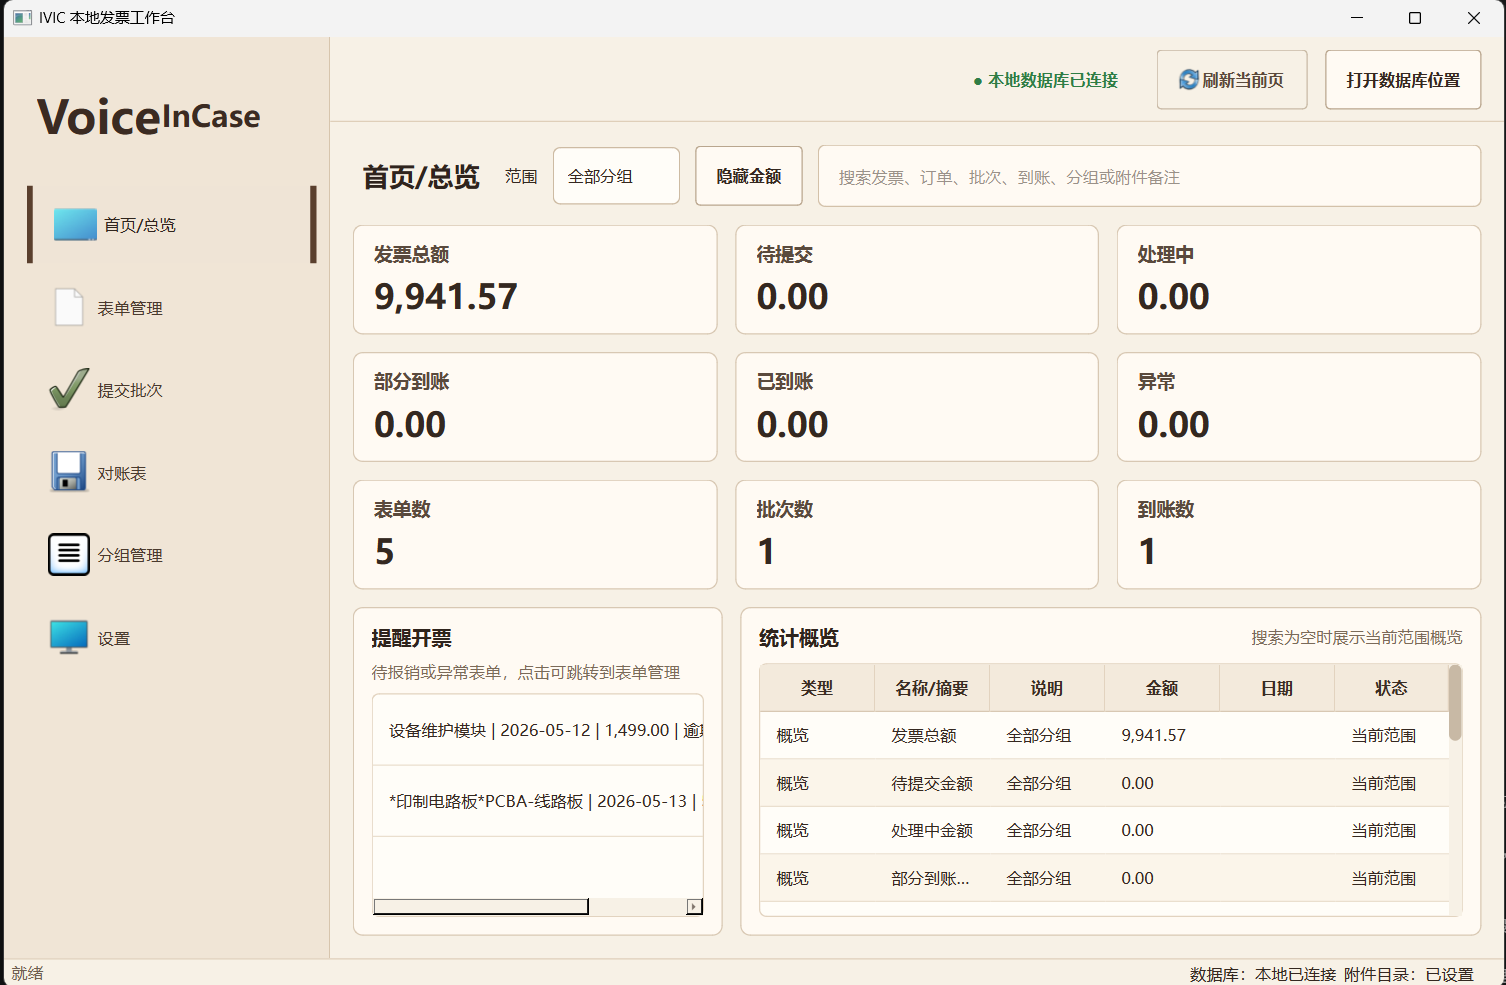
\includegraphics[width=0.92\linewidth]{page1.png}
  \caption{v2.0.x 实际首页：业务结构接近预期，但仍有明显 Qt 控件式痕迹}
  \label{fig:v20-page1}
\end{figure}

\begin{figure}[H]
  \centering
  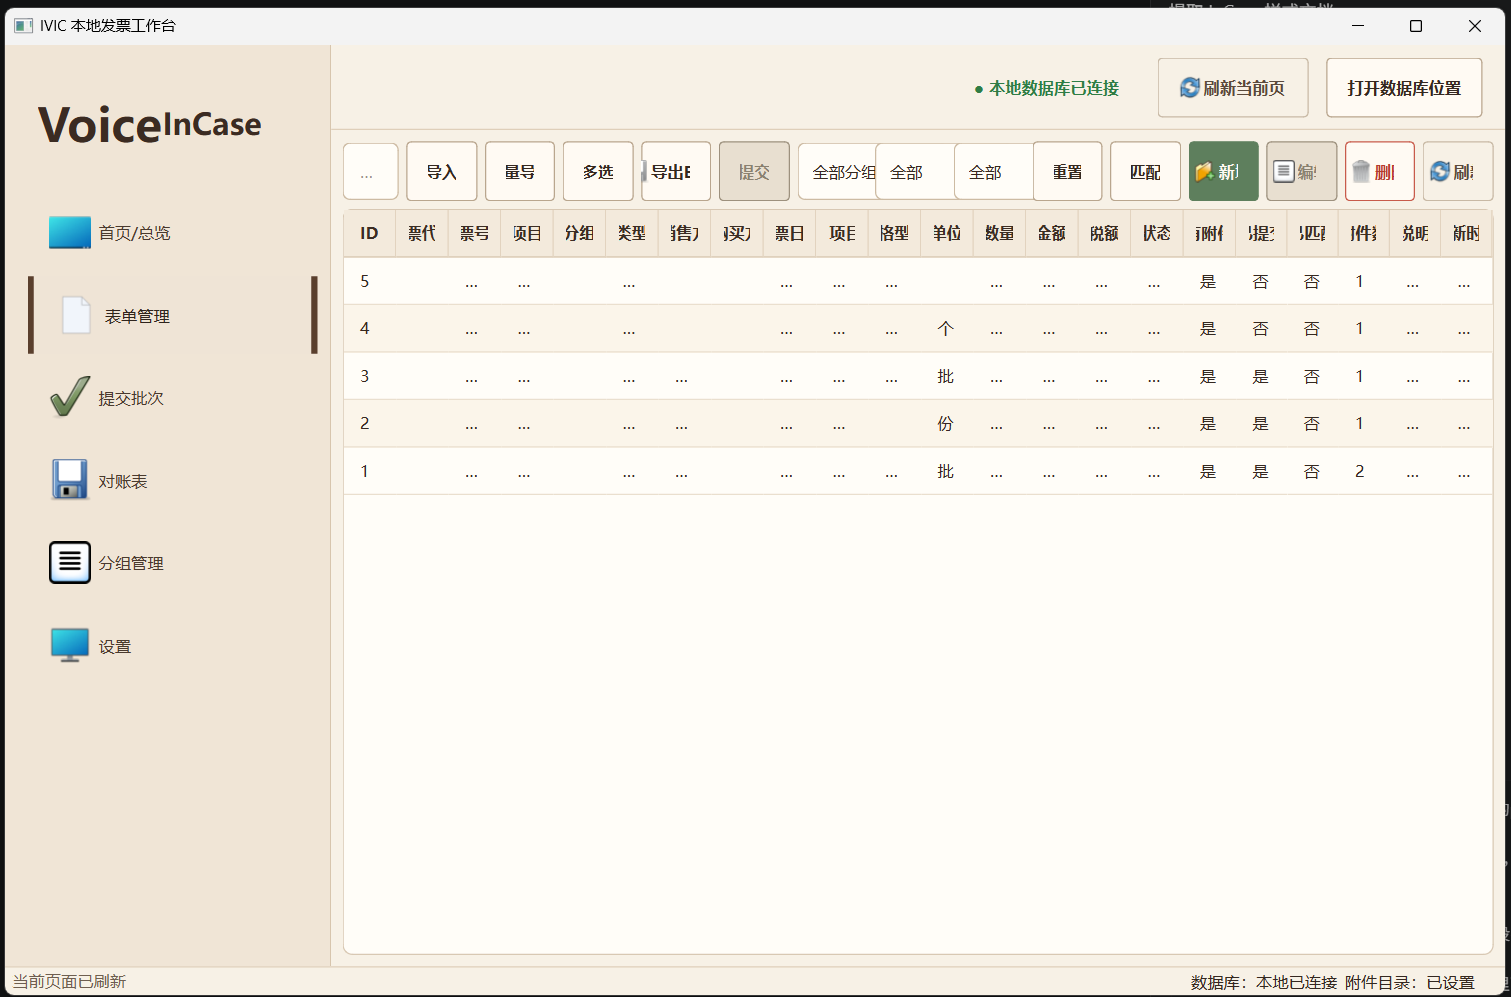
\includegraphics[width=0.92\linewidth]{page2.png}
  \caption{v2.0.x 实际表单页：按钮、表头、列宽和图标体系难以支撑目标质感}
  \label{fig:v20-page2}
\end{figure}

\subsection{v2.0.x 暴露的问题}

\begin{longtable}{p{3.4cm}p{11.0cm}}
\toprule
问题类别 & 表现 \\
\midrule
视觉一致性 & 图标来源不统一，按钮与表格像系统默认控件，品牌气质与 InCase 指南差距明显。 \\
布局弹性 & 工具栏按钮容易截断，表格字段横向挤压，主从表布局缺少现代桌面应用的密度控制。 \\
组件复用 & PyQt 页面主要以 Python 文件同级堆叠，控件样式、状态、交互逻辑难以像 React 组件一样拆分复用。 \\
样式迭代 & QSS 能做基础美化，但复杂状态、主题 token、表格细节、弹窗反馈和响应式布局难以长期维护。 \\
工程边界 & UI、事件处理、数据调用和页面状态容易混在同一文件，单文件行数膨胀后理解成本过高。 \\
长期演进 & OCR、PDF 预览、附件管理、导出模板、备份恢复、数据迁移等本地能力需要更清晰的前后端边界。 \\
\bottomrule
\end{longtable}

\subsection{v2.1.x 版本目标}

\begin{itemize}
  \item \req{VG-01} 保留 v2.0.x 已确认的核心业务和页面结构，不因技术栈迁移推翻需求。
  \item \req{VG-02} 使用 Tauri 2 + React + TypeScript 实现可维护、可组件化的桌面 UI。
  \item \req{VG-03} 使用 Rust 命令层处理 SQLite、文件导入、附件复制、路径校验、备份恢复和迁移。
  \item \req{VG-04} 按 InCase 样式指南建立桌面 token、组件规范和截图验收规则。
  \item \req{VG-05} 工程结构必须分层清晰，避免单个 UI 目录下堆大量同级页面文件。
  \item \req{VG-06} 开发流程中应善用子智能体做并行审阅和专项验证，但必须保持主线集成清晰。
\end{itemize}

\section{产品定位}

\subsection{产品愿景}

IVIC 是一款个人离线桌面发票工作台。它服务于“我需要看清自己的发票、订单、报销批次、分组归属和到账状态”的个人场景，而不是多人在线协同财务系统。应用的核心价值是：在不上传隐私数据、不依赖服务器的前提下，把分散的发票 PDF、订单文本、截图附件、报销批次和到账流水组织成可查询、可追踪、可对账的本地资料库。

v2.1.x 的产品愿景可以概括为：

\begin{quote}
  用现代桌面技术重做 IVIC 的壳和前端，让 v2.0.x PDR 中“应该长什么样、应该怎么用”的设计终于能够被稳定实现。
\end{quote}

\subsection{目标用户}

\begin{itemize}
  \item 经常需要个人垫付、收集发票、提交报销、等待到账的学生、科研人员、实验室成员或个人项目维护者。
  \item 需要把不同发票交给不同负责人、不同分组或不同场景处理的用户。
  \item 需要在本地保留发票原件、截图附件、批次说明和到账记录的人。
  \item 不希望使用联网 SaaS、不希望将发票和银行截图上传到外部服务的人。
\end{itemize}

\subsection{产品边界}

\begin{longtable}{p{4.0cm}p{10.4cm}}
\toprule
范围类别 & 说明 \\
\midrule
必须覆盖 & 首页/总览、表单管理、单条/批量导入、发票与订单匹配、提交批次、到账交易、到账对账、分组管理、设置、备份恢复。 \\
必须本地化 & 数据库、附件、发票 PDF、截图、配置文件和迁移日志均保存于本地。 \\
不是网站 & Tauri 只是桌面壳和本地能力承载，不提供服务器，不设计为浏览器访问的网站后台。 \\
不作为 v2.1.x 目标 & 多用户权限、云同步、在线审批流、真实财务系统直连、自动网银拉取流水、企业级审计合规。 \\
可预留扩展 & 本地 OCR 增强、PDF 预览优化、导出模板、InCase 生态内应用跳转、数据包导入导出。 \\
\bottomrule
\end{longtable}

\section{总体设计原则}

\subsection{本地优先}

\begin{itemize}
  \item \req{PR-01} IVIC \must{}在无网络环境下完成主要功能，包括导入、编辑、查询、匹配、批次管理、对账和导出。
  \item \req{PR-02} 应用不得默认上传发票、附件、银行截图、数据库或使用统计。
  \item \req{PR-03} 检测更新、远程文档或其他联网能力必须由用户显式启用，并清楚说明会访问网络。
  \item \req{PR-04} 数据库配置应抽象为“选择本地数据文件和附件目录”，用户不应被迫理解服务器、端口或连接串。
\end{itemize}

\subsection{面向个人真实流程}

\begin{itemize}
  \item \req{PR-05} 系统应允许用户先粗略导入，再通过表格、详情面板、匹配流程逐步修正。
  \item \req{PR-06} 系统应表达现实中的不整齐状态：部分到账、金额差异、材料缺失、异常结项和人工备注。
  \item \req{PR-07} 分组、标签、分类、状态应优先服务个人检索和归集，不引入企业级主数据维护负担。
\end{itemize}

\subsection{组件化桌面 UI}

\begin{itemize}
  \item \req{PR-08} v2.1.x 前端\must{}由 React 组件构成，页面、工具栏、表格、详情面板、弹窗、状态标签等应可复用。
  \item \req{PR-09} UI 风格\must{}以 InCase 样式指南为准，避免 Qt 默认控件感、系统图标混用和表格字段硬挤。
  \item \req{PR-10} 设计应像桌面应用，而不是普通网页后台：左侧导航、顶部工具栏、主数据区、右侧详情/上下文面板应形成稳定工作台。
\end{itemize}

\subsection{工程可维护}

\begin{itemize}
  \item \req{PR-11} 页面、组件、服务、类型、样式、后端命令必须分层组织，不允许把页面逻辑集中堆在少数超长文件里。
  \item \req{PR-12} 单文件代码量应受控；超出阈值时优先拆分为子组件、hooks、service、type 或 Rust 子模块。
  \item \req{PR-13} 数据访问、文件操作、路径安全、备份恢复、迁移逻辑应由 Rust 命令层承担，前端不得直接拼装本地文件系统副作用。
\end{itemize}

\section{品牌与视觉规范}

\subsection{品牌资产}

IVIC v2.1.x \must{}使用 \texttt{misc/logo/IVIC\_Logo.png} 作为官方 logo 来源。logo 可用于文档标题页、应用欢迎区、关于页、安装包图标设计参考和设置页品牌信息。

\begin{figure}[H]
  \centering
  
\includegraphics[width=0.48\linewidth]{IVIC_Logo.png}
  \caption{IVIC logo：纳入 v2.1.x PDR 与后续应用品牌资产}
  \label{fig:ivic-logo}
\end{figure}

由于 logo 本身偏蓝紫与金属质感，应用 UI 不应简单复制 logo 色彩。界面主风格仍以 InCase 样式指南中的暖米、胡桃木、牛皮纸边框、硬阴影为基础，并可用暗绿色作为关键操作强调色。

\subsection{InCase 风格复用}

InCase 当前主风格可概括为“木质收纳 / 牛皮纸盒 / 半扁平积木感 / 工具型库存系统”。IVIC 是发票管理工具，应复用其工具感和硬边界，而不是做成柔雾渐变或通用 SaaS 后台。

\begin{figure}[H]
  \centering
  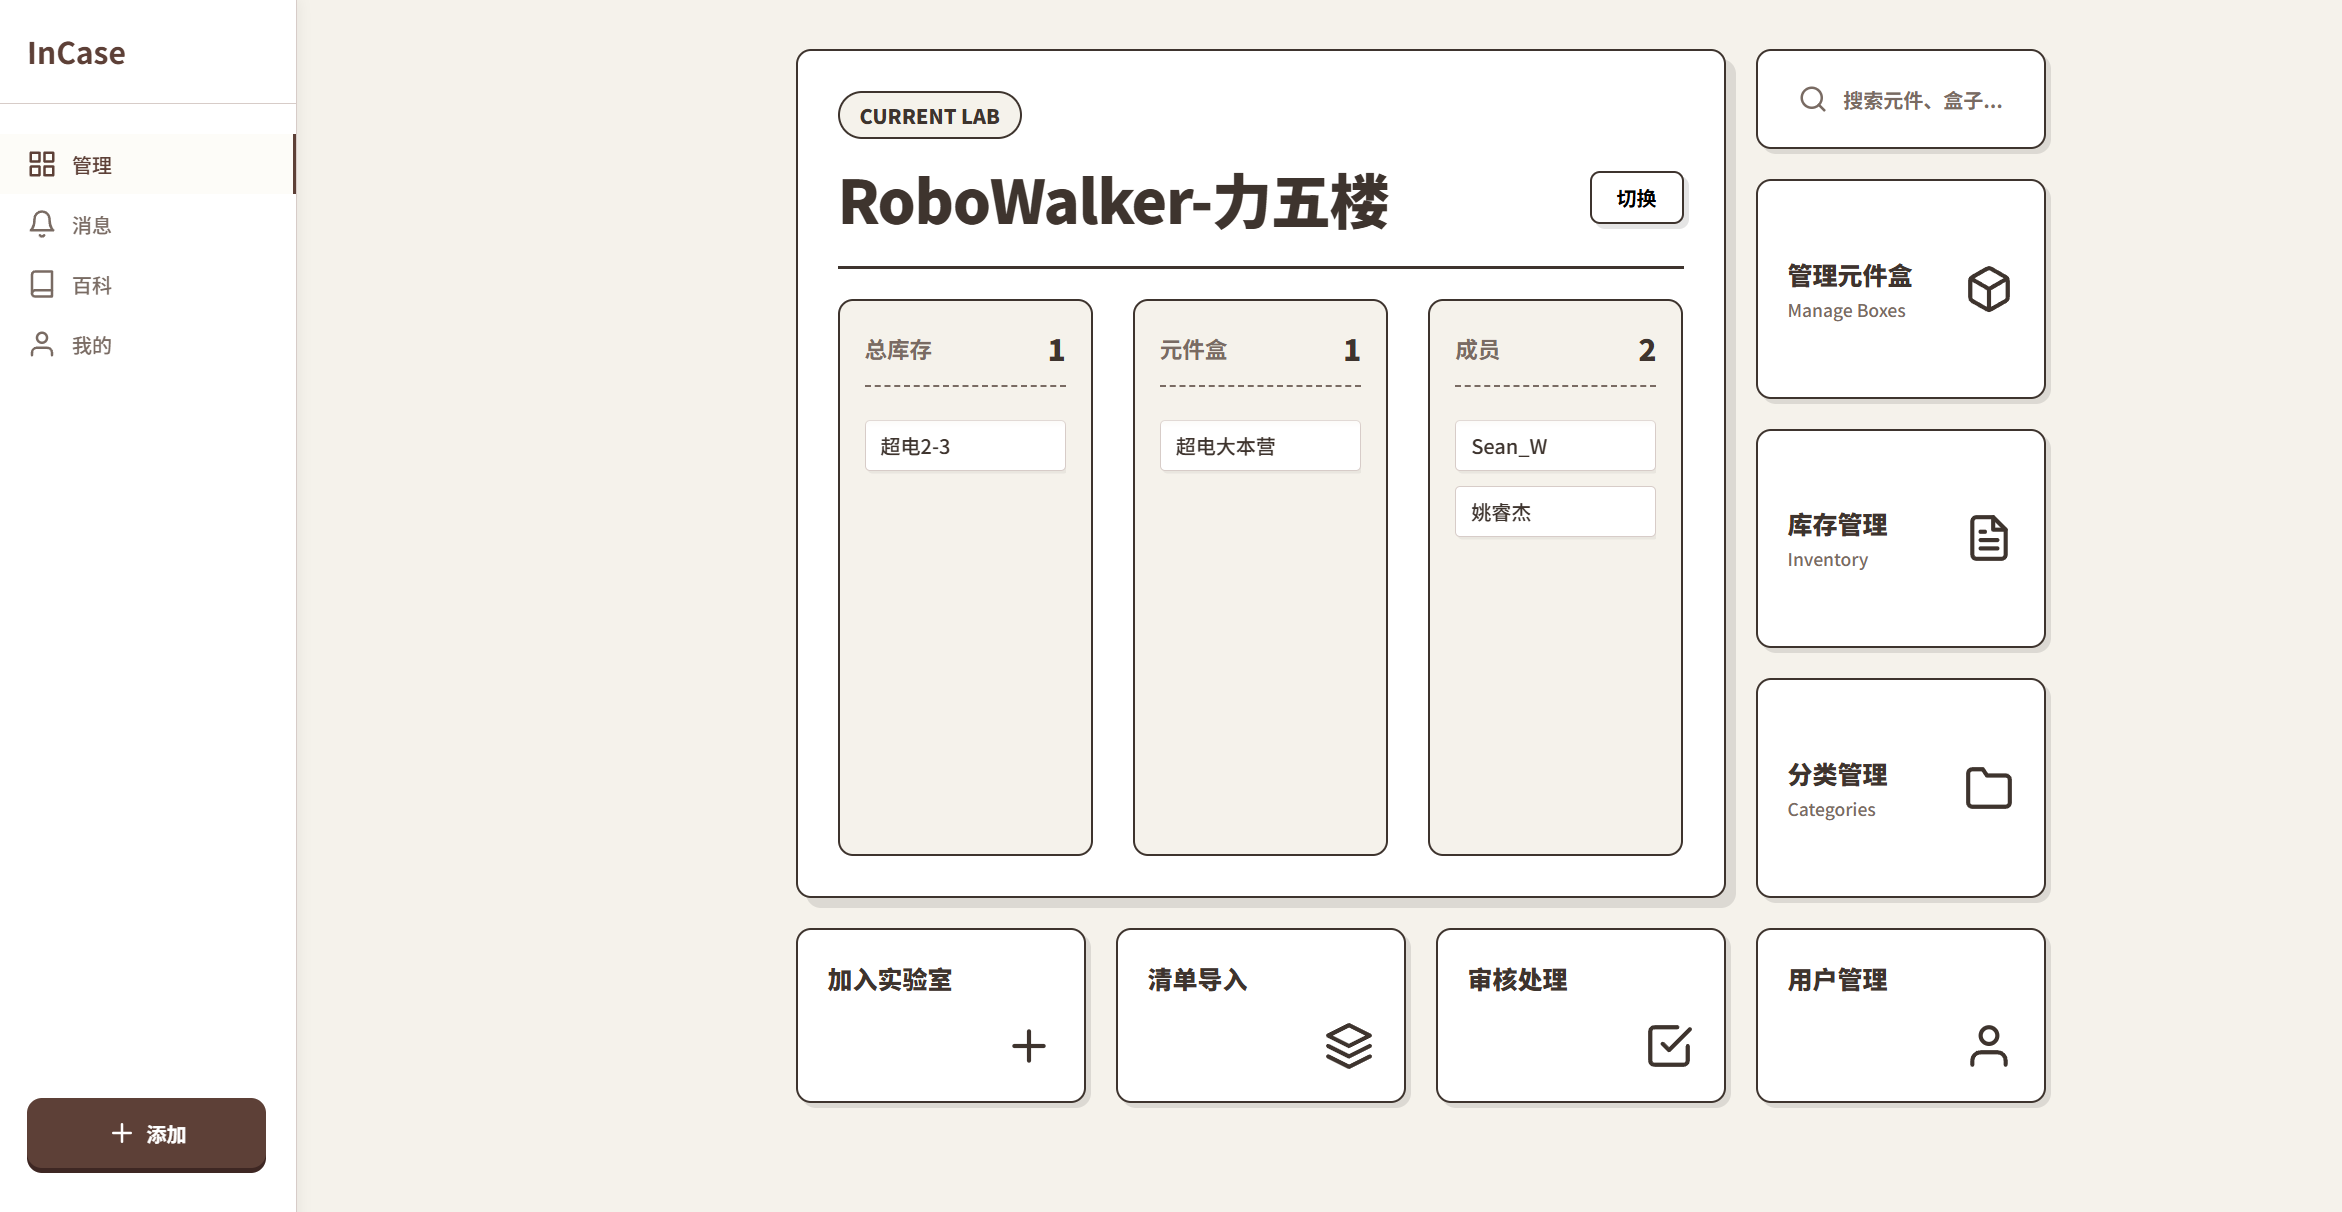
\includegraphics[width=0.92\linewidth]{incase-1.png}
  \caption{InCase 风格参考：侧栏、硬边框、低饱和暖色工作台}
  \label{fig:incase-style-1}
\end{figure}

\begin{figure}[H]
  \centering
  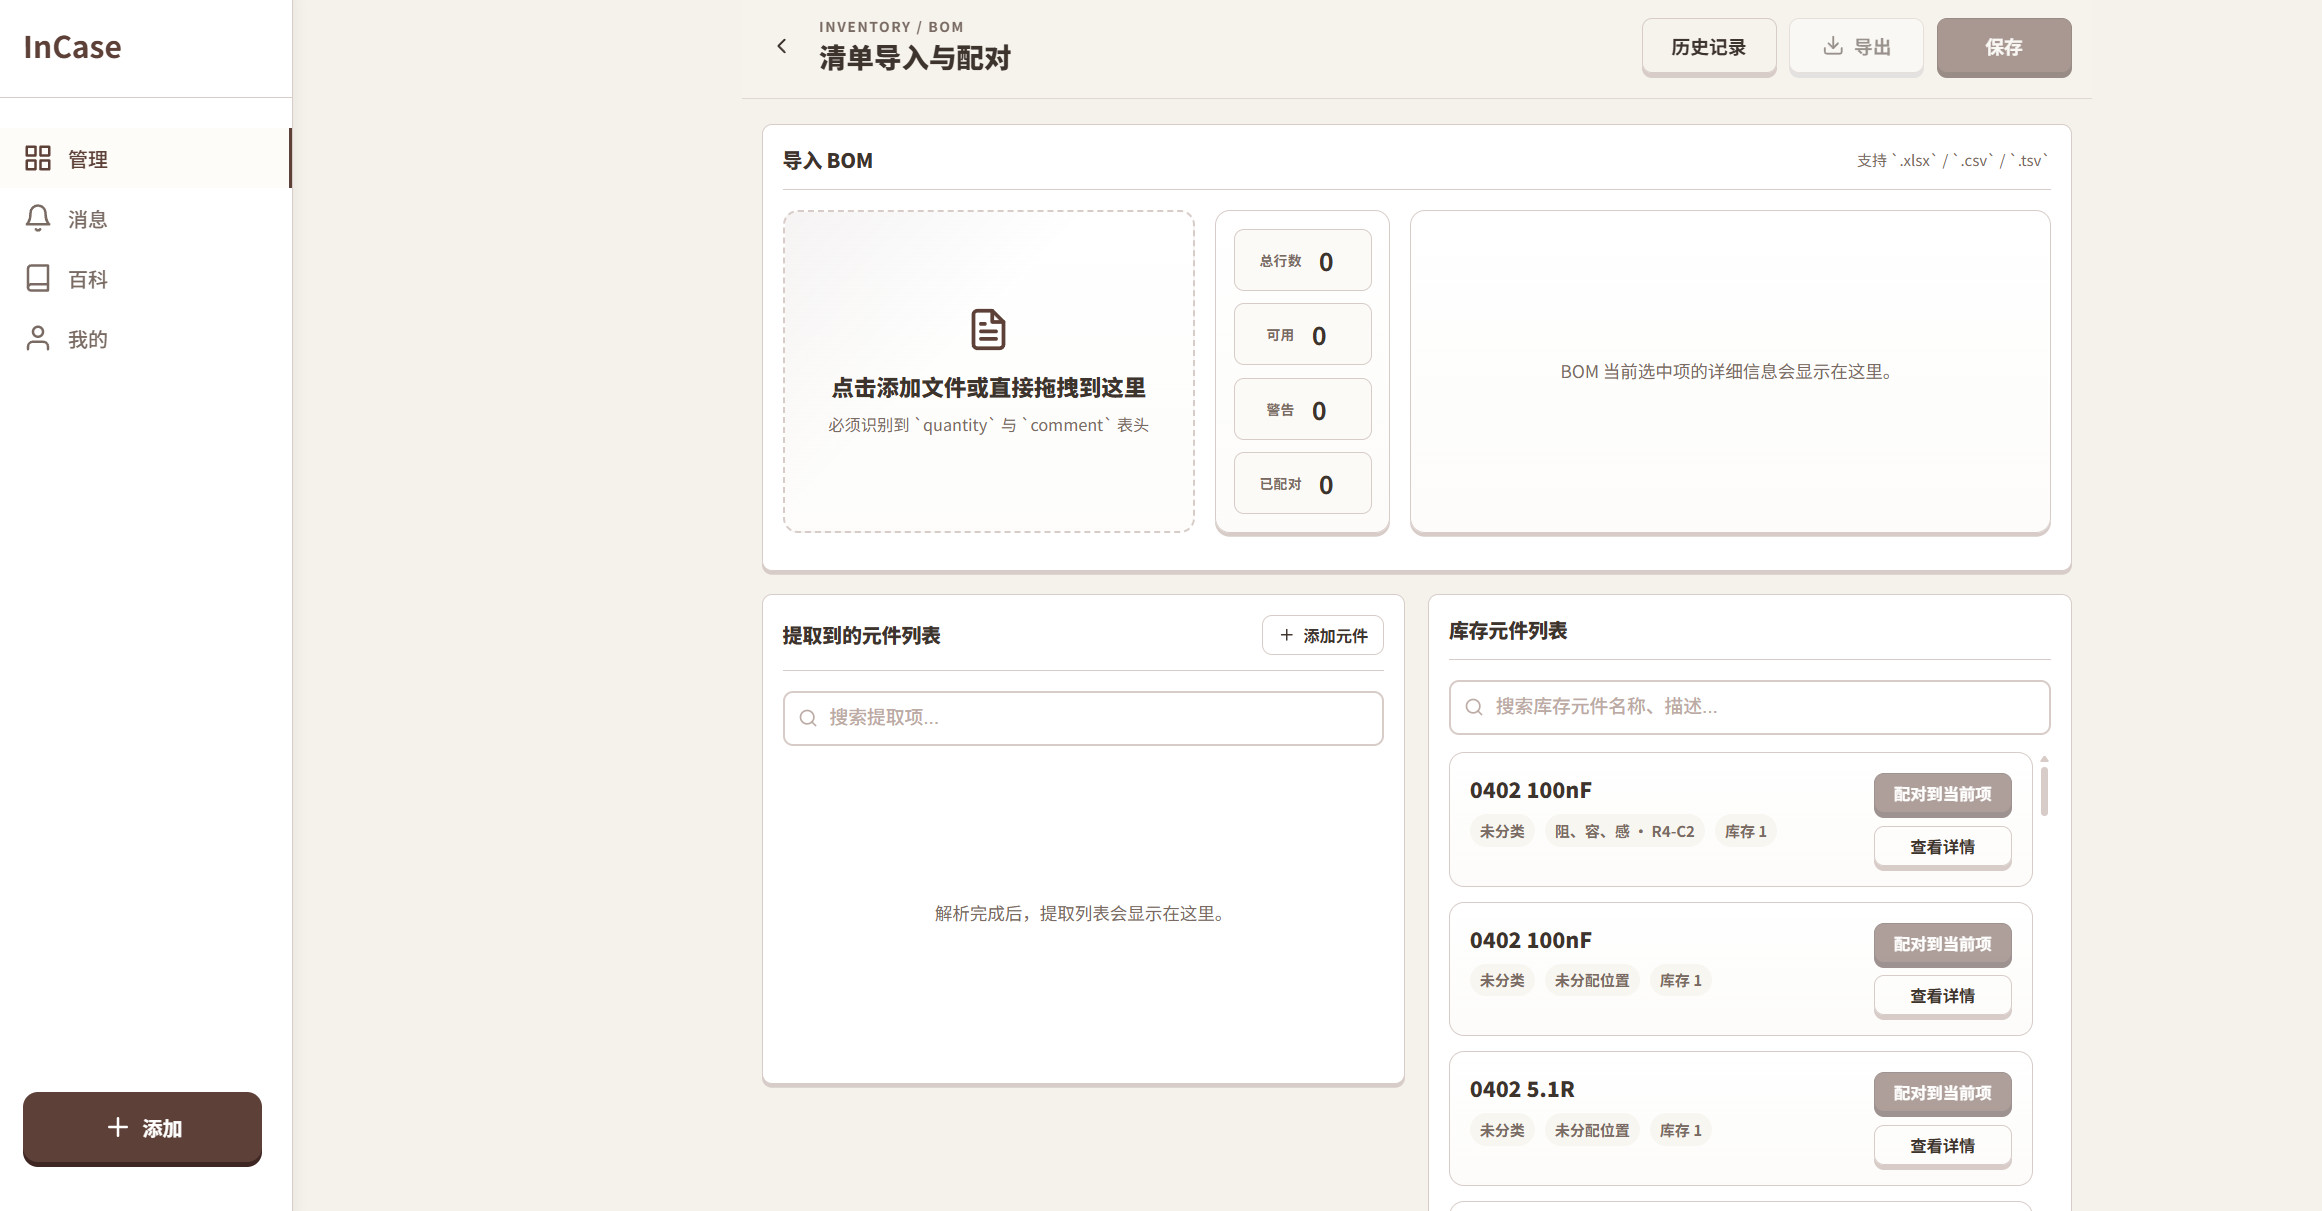
\includegraphics[width=0.92\linewidth]{incase-4.png}
  \caption{InCase 风格参考：导入、统计、预览与候选列表组合工作流}
  \label{fig:incase-style-4}
\end{figure}

\subsection{设计 token}

v2.1.x 前端应在 CSS Variables 中建立最小 token 集，并让组件全部通过 token 引用颜色、圆角、阴影和字体。

\begin{longtable}{p{4.0cm}p{4.0cm}p{6.4cm}}
\toprule
Token & 建议值 & 用途 \\
\midrule
\texttt{--color-primary} & \texttt{\#5D4037} & 胡桃木主色，主按钮、高亮、主图标。 \\
\texttt{--color-primary-dark} & \texttt{\#3E2723} & 深咖啡，按钮硬阴影和深色边界。 \\
\texttt{--color-action} & \texttt{\#2F5D50} & 暗绿色操作色，用于保存、创建、已连接等状态。 \\
\texttt{--color-border} & \texttt{\#D7CCC8} & 牛皮纸边框、分割线、浅硬阴影。 \\
\texttt{--bg-app} & \texttt{\#F5F2EB} & 应用背景，低饱和暖米色。 \\
\texttt{--bg-surface} & \texttt{\#FFFFFF} & 卡片、弹窗、输入框内容面。 \\
\texttt{--text-main} & \texttt{\#3E342E} & 主文字。 \\
\texttt{--text-secondary} & \texttt{\#796B63} & 次级说明、辅助文字。 \\
\texttt{--radius-sm/md/lg} & \texttt{4px / 8px / 12px} & 小标签、按钮/输入、弹窗/大模块。 \\
\texttt{--shadow-card} & \texttt{0 3px 0 \#D7CCC8} & 卡片硬阴影。 \\
\texttt{--shadow-btn} & \texttt{0 4px 0 \#3E2723} & 按钮下沉阴影。 \\
\bottomrule
\end{longtable}

\subsection{组件风格要求}

\begin{itemize}
  \item 按钮：主按钮使用胡桃木或暗绿色底，深色硬阴影，按下时通过 \texttt{translateY} 下沉。
  \item 卡片：白底、牛皮纸边框、硬阴影；半径以 8px 为主，不滥用胶囊圆角。
  \item 输入框：2px 边框，聚焦只改变边框色，不使用强发光。
  \item 表格：强调可读性，提供列宽、排序、筛选、列显示控制和稳定横向滚动。
  \item 标签：状态标签应小而清楚，金额、ID 和统计数字可使用等宽字体。
  \item 弹窗：黑褐色边框、硬投影、短促 pop 动效；避免系统默认对话框。
  \item 图标：优先使用线性图标体系，跟随 \texttt{currentColor}；不要混用系统图标和随机图片图标。
\end{itemize}

\section{信息架构}

v2.1.x 页面结构延续 v2.0.x PDR 的主导航，不以 \texttt{project-overview.md} 中旧 PyQt 页面为准，也不照搬通用网页后台。主导航至少包含：

\begin{enumerate}
  \item 首页 / 总览 Dashboard
  \item 表单管理 Form Workspace
  \item 提交批次 Reimbursement Batches
  \item 对账表 Reconciliation
  \item 分组管理 Groups
  \item 设置 Settings
\end{enumerate}

\subsection{通用桌面布局}

典型页面采用以下结构：

\begin{itemize}
  \item 左侧固定导航栏：品牌、主模块、状态入口。
  \item 顶部工具栏：页面标题、全局搜索、筛选、刷新、主要操作。
  \item 中央数据区：表格、卡片、主从表、统计视图或导入预览。
  \item 右侧详情面板：当前选中对象详情、附件、状态日志、上下文操作。
  \item 弹窗/抽屉：新增、编辑、批量导入、匹配、对账、确认操作。
  \item 底部状态提示：数据库状态、最近保存结果、导入错误和迁移状态。
\end{itemize}

\subsection{首页 / 总览}

首页用于呈现全局状态、提醒和快速检索结果。v2.1.x 的视觉目标继续参考 v2.0.x PDR 草图，而不是 v2.0.x 实际 PyQt 截图。

\begin{figure}[H]
  \centering
  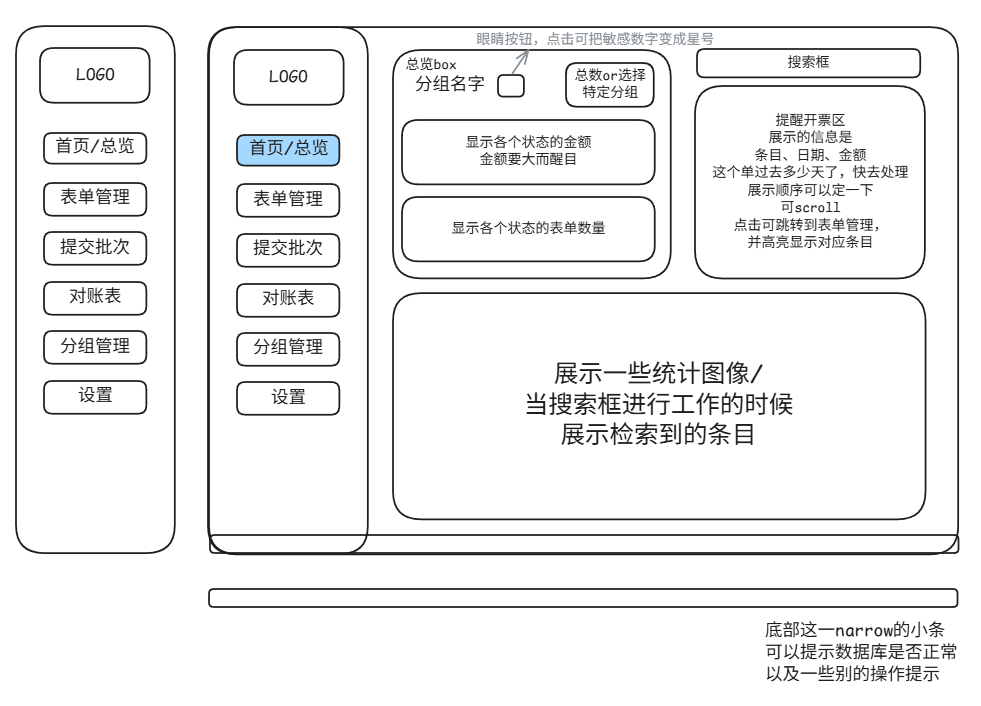
\includegraphics[width=0.92\linewidth]{mainpage.png}
  \caption{首页/总览目标草图：v2.1.x 继续保留该业务布局}
  \label{fig:mainpage}
\end{figure}

首页应包含：分组范围切换、敏感金额隐藏、金额统计、数量统计、提醒开票、搜索结果、统计概览和状态反馈。

\subsection{表单管理}

\begin{figure}[H]
  \centering
  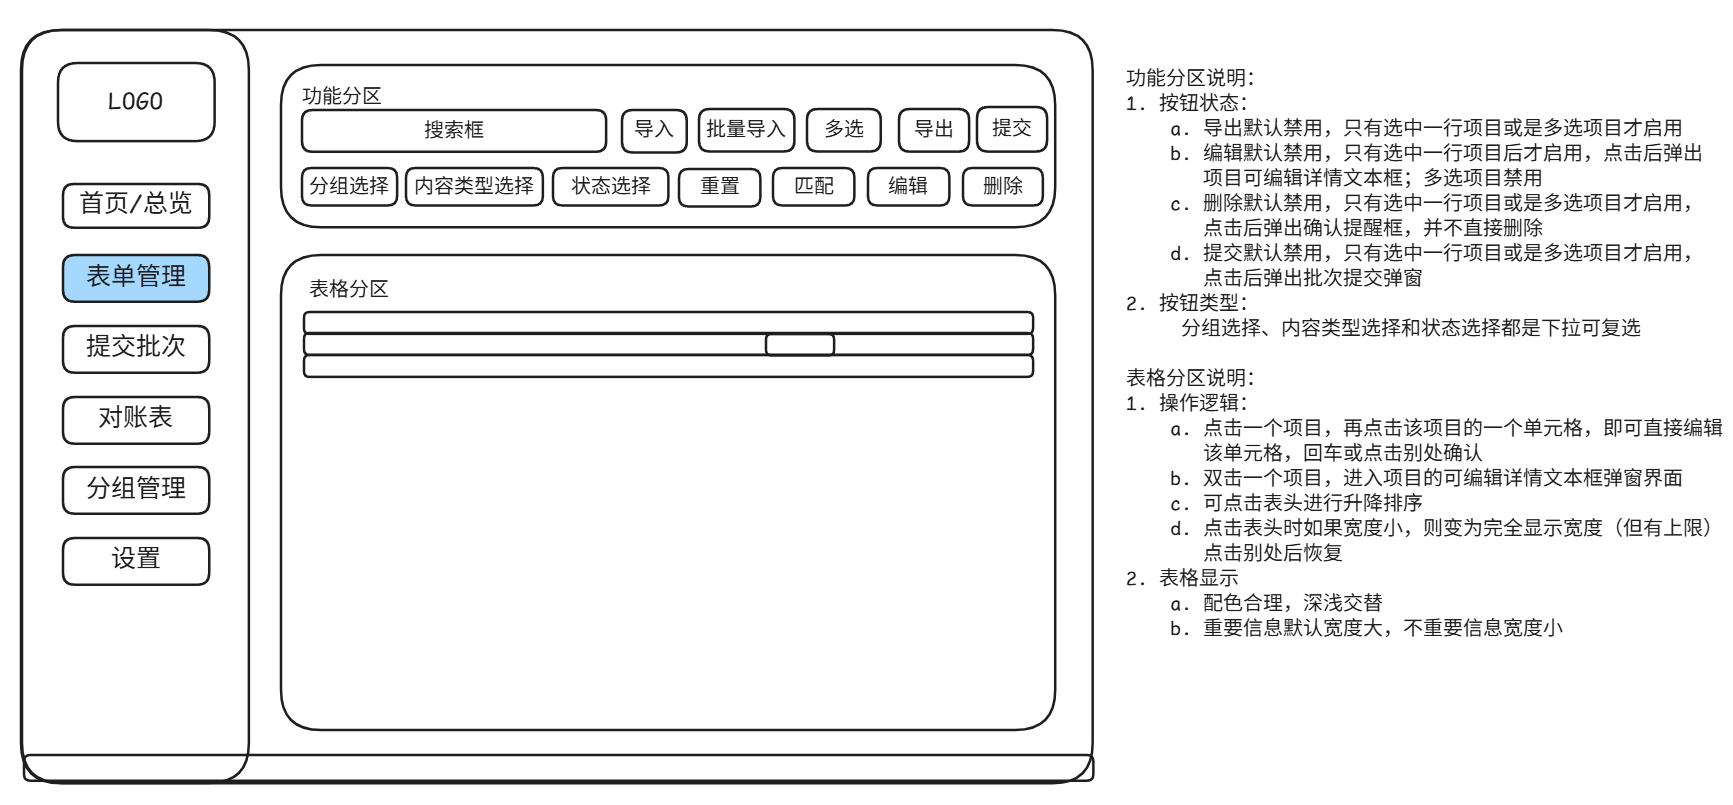
\includegraphics[width=0.92\linewidth]{sheetmanage.png}
  \caption{表单管理目标草图：v2.1.x 需用现代 React 表格和详情面板实现}
  \label{fig:sheetmanage}
\end{figure}

表单管理是发票、订单和附件的统一工作区。v2.1.x \must{}避免把所有操作按钮平铺挤在同一行；常用操作放工具栏，低频操作进入更多菜单或上下文面板。表格必须支持列宽、列显示、排序、筛选、批量选择和详情抽屉。

\subsection{单条导入与批量导入}

\begin{figure}[H]
  \centering
  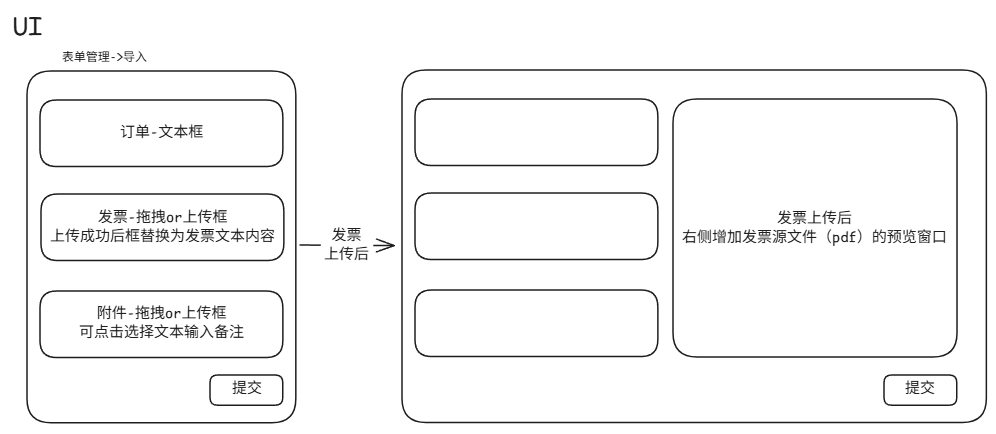
\includegraphics[width=0.88\linewidth]{addui.png}
  \caption{单条导入目标草图：订单文本、发票文件、附件备注与 PDF 预览}
  \label{fig:addui}
\end{figure}

\begin{figure}[H]
  \centering
  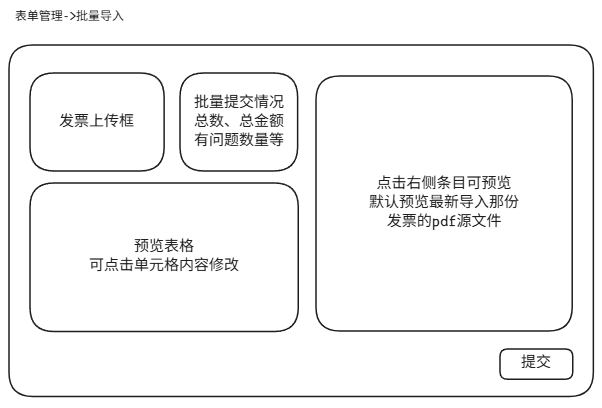
\includegraphics[width=0.80\linewidth]{addui-batch.png}
  \caption{批量导入目标草图：多文件、识别结果预览、问题修正和当前 PDF 预览}
  \label{fig:adduibatch}
\end{figure}

导入流程应采用“先暂存预览，再确认入库”的模式。前端负责可编辑预览、错误标记、当前 PDF 预览与批量修正；Rust 命令层负责文件复制、路径校验、解析任务调度和数据库事务。

\subsection{提交批次}

\begin{figure}[H]
  \centering
  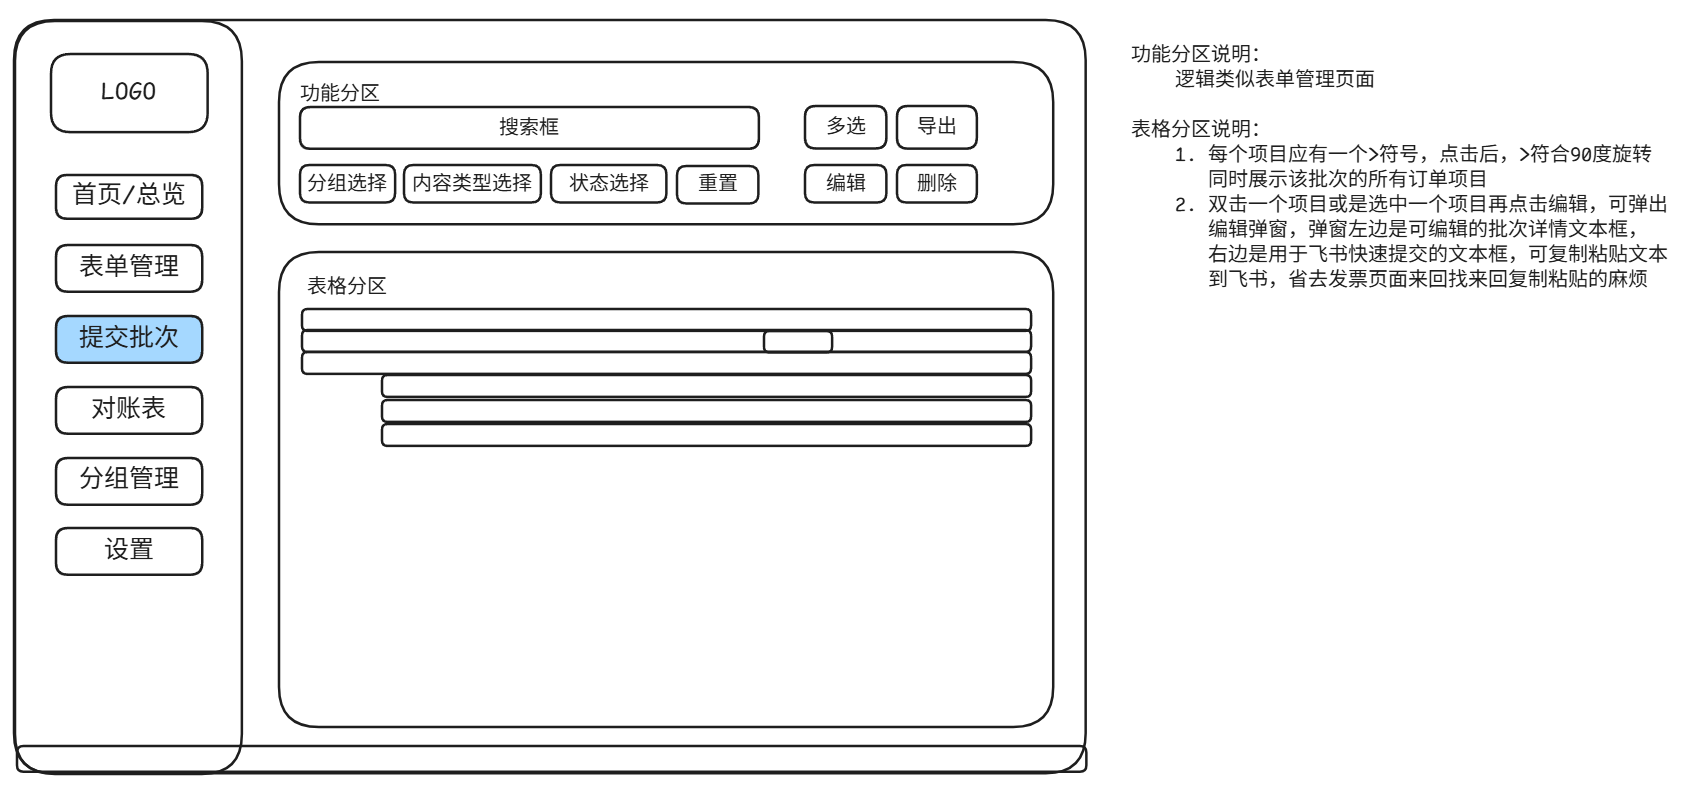
\includegraphics[width=0.92\linewidth]{batchsubmit.png}
  \caption{提交批次目标草图：批次、子订单、发票和快速提交文本}
  \label{fig:batchsubmit}
\end{figure}

提交批次页继续保留 v2.0.x 的主从结构：上方批次列表，下方子订单/发票/日志 Tab 或详情面板。React 实现应支持展开行、右侧详情、状态标签和批量操作，而不是简单复制 Qt 双表格。

\subsection{对账表}

\begin{figure}[H]
  \centering
  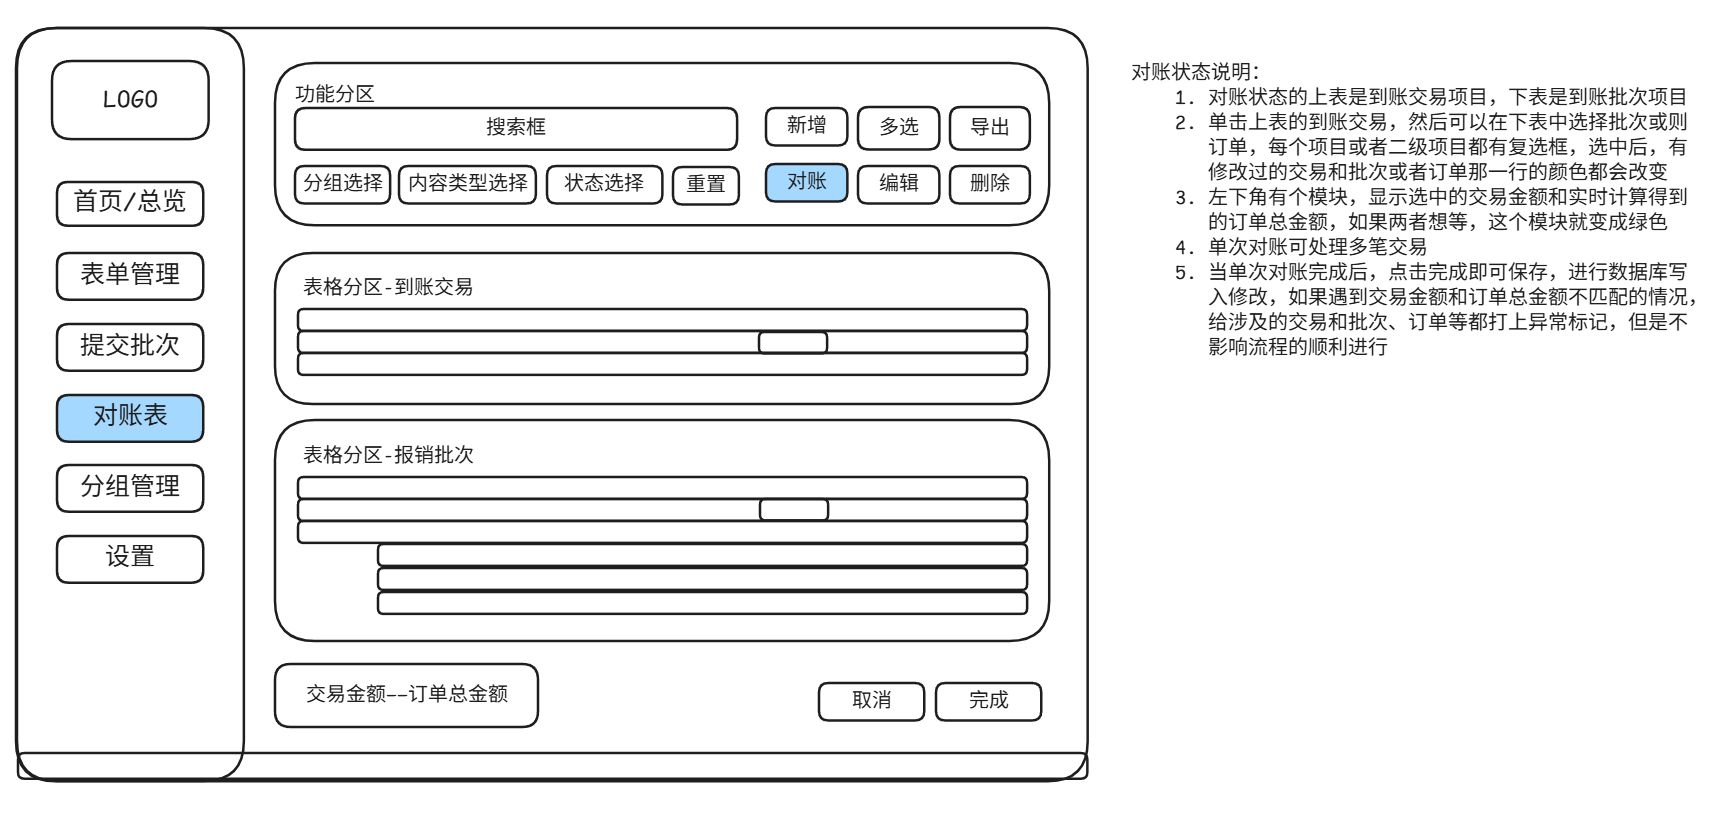
\includegraphics[width=0.92\linewidth]{incomesheetmatching.png}
  \caption{到账对账目标草图：交易、批次、子订单的多级匹配}
  \label{fig:reconciliation}
\end{figure}

对账表用于把到账交易与报销批次或子订单建立匹配。v2.1.x 应提供清晰的金额差异提示、临时匹配状态、撤销、完成写库和附件入口。

\subsection{分组管理与设置}

\begin{figure}[H]
  \centering
  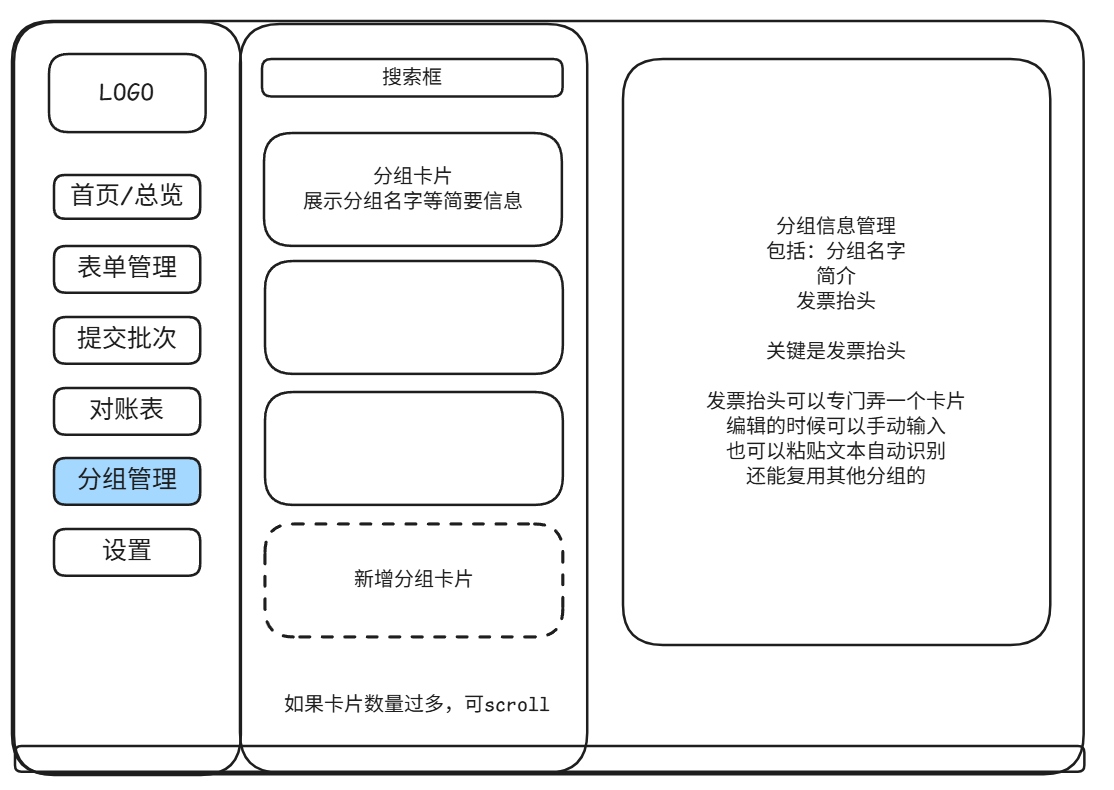
\includegraphics[width=0.92\linewidth]{groupmanage.png}
  \caption{分组管理目标草图：左侧分组卡片，右侧详情编辑}
  \label{fig:group}
\end{figure}

\begin{figure}[H]
  \centering
  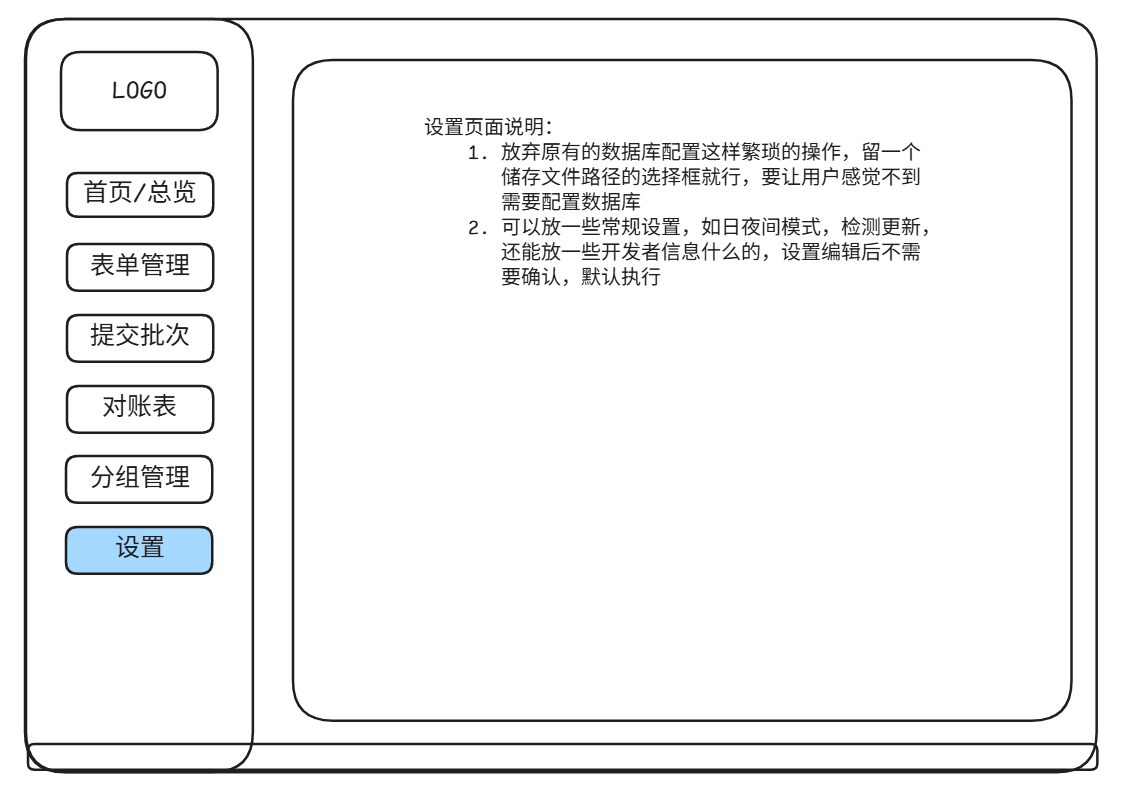
\includegraphics[width=0.88\linewidth]{settings.png}
  \caption{设置页目标草图：本地数据库、附件目录、显示模式和更新开关}
  \label{fig:settings}
\end{figure}

分组管理保留左列表右详情结构。设置页应隐藏复杂数据库细节，只暴露本地数据库文件、附件目录、备份恢复、主题设置、更新检测和关于信息。

\section{核心业务对象}

\subsection{对象定义}

v2.1.x 继续沿用 v2.0.x 的真实业务模型，同时以英文 domain 名称建立 TypeScript 与 Rust 类型。

\begin{longtable}{p{3.2cm}p{4.0cm}p{7.2cm}}
\toprule
中文对象 & 领域名称 & 说明 \\
\midrule
发票 & Invoice & 票据本身，包含金额、日期、销售方/购买方文本、原始文件和识别文本。 \\
订单 / 表单条目 & Order / FormItem & 可与发票匹配的业务条目，也可表示待开票、非发票费用或导入文本。 \\
附件 & Attachment & 发票原件、银行截图、聊天记录、财务系统截图和补充材料。 \\
报销批次 & ReimbursementBatch & 一次提交给财务、负责人或学校系统的一组材料。 \\
报销子订单 & ReimbursementItem & 批次内部可独立跟踪、对账和异常结项的最小条目。 \\
到账交易 & ReconciliationTransaction & 银行到账、退款、冲销或其他资金流水。 \\
对账匹配 & ReconciliationMatch & 到账交易与批次/子订单之间的匹配关系。 \\
分组 & ExpenseGroup & 负责人、交接对象、场景、比赛、实验室或发票抬头规则。 \\
标签 & Tag & 用户自定义轻量标记，用于筛选、搜索和批量整理。 \\
分类 & Category & 比标签更稳定的业务分类，如报销到账、退款、采购、差旅、材料。 \\
往来方 & Counterparty & 不恢复独立供应商主数据；仅作为发票销售方/购买方文本概念或未来轻量字典。 \\
状态 & Status & 发票、子订单、批次、交易等对象的状态枚举。 \\
系统设置 & Settings & 数据库路径、附件目录、主题、更新检测、备份策略等本地配置。 \\
\bottomrule
\end{longtable}

\subsection{数据结构原则}

\begin{itemize}
  \item 删除或不恢复独立 \texttt{supplier} 主数据维护，发票表保存销售方名称、销售方税号等文本字段。
  \item 删除或不继续暴露 \texttt{project.budget\_amount}，项目只作为归属和统计维度。
  \item 新增或保留 \texttt{expense\_group}，作为个人归集、负责人、场景和抬头识别的核心对象。
  \item 使用 \texttt{reimbursement\_item} 表达批次内部子订单状态，不再只靠批次单状态表达全部流程。
  \item 使用 \texttt{reconciliation\_transaction} 与 \texttt{reconciliation\_match} 支持到账对账和金额差异。
  \item 附件应逐步演进为通用附件模型，至少支持备注、所属对象、相对路径和文件哈希。
\end{itemize}

\subsection{状态模型}

\begin{longtable}{p{3.2cm}p{4.4cm}p{6.8cm}}
\toprule
对象 & 状态 & 含义 \\
\midrule
发票/订单 & 待开票、待匹配、已匹配、待提交、已提交、已取消、异常 & 表达票据采集与提交前流程。 \\
报销子订单 & 待提交、已提交、审核中、待补充、部分到账、已到账、已驳回、异常结项、已取消 & 表达批次内部条目的真实处理进度。 \\
报销批次 & 待提交、已提交、处理中、部分到账、部分完成、已完成、需处理、异常结项、已取消 & 由子订单状态聚合得到，也允许人工备注说明。 \\
到账交易 & 待对账、部分对账、已对账、异常 & 由匹配金额与交易金额关系推导。 \\
\bottomrule
\end{longtable}

\section{数据需求}

\subsection{本地数据目录}

v2.1.x 以 SQLite 作为正式本地数据库，不再把 MySQL 作为普通用户运行路径。应用首次启动时应在系统推荐的用户数据目录下创建默认数据空间，具体目录由 Tauri/Rust 根据平台解析，不应在代码或文档中写死开发者本机路径。

\begin{longtable}{p{4.0cm}p{10.4cm}}
\toprule
数据类型 & 要求 \\
\midrule
SQLite 数据库 & 默认保存在应用用户数据目录；用户可在设置页选择或迁移到其他本地路径。 \\
附件目录 & 默认位于用户数据目录下，保存发票原件、截图、PDF、补充材料和导出中间文件。 \\
配置文件 & 保存主题、最近路径、更新检测开关、窗口状态和隐私偏好。 \\
备份文件 & 由用户显式创建，包含数据库和必要附件索引；恢复前必须提示影响范围。 \\
迁移日志 & 记录 schema version、迁移时间、迁移结果、错误信息和备份位置。 \\
\bottomrule
\end{longtable}

\subsection{Schema Version 与迁移}

\begin{itemize}
  \item \req{DR-MIG-01} SQLite 数据库\must{}包含 schema version 记录，用于判断当前数据库结构是否需要迁移。
  \item \req{DR-MIG-02} 每次结构变更\must{}提供可追踪迁移脚本或 Rust migration 函数，并记录迁移日志。
  \item \req{DR-MIG-03} 迁移前\must{}自动创建原数据库备份；迁移失败时不得覆盖原数据库。
  \item \req{DR-MIG-04} 旧 PyQt 数据迁移\must{}处理 supplier 到 invoice seller 文本字段的回填。
  \item \req{DR-MIG-05} 旧预算字段\should{}从 UI 移除；数据库层可分阶段迁移，但不得继续作为核心统计来源。
\end{itemize}

\subsection{目标数据表}

\begin{longtable}{p{4.4cm}p{10.0cm}}
\toprule
表名 & 说明 \\
\midrule
\texttt{schema\_version} & 当前数据库结构版本和最近迁移记录。 \\
\texttt{project} & 项目/活动/课题等上层归属，弱化预算控制。 \\
\texttt{expense\_group} & 分组、负责人、场景、发票抬头规则。 \\
\texttt{invoice} & 发票主体信息，包含金额、日期、销售方/购买方文本字段、文件路径。 \\
\texttt{order\_item} & 订单或待开票条目，可与发票匹配。 \\
\texttt{attachment} & 通用附件，保存 owner、文件名、相对路径、类型、备注和哈希。 \\
\texttt{reimbursement} & 报销批次。 \\
\texttt{reimbursement\_item} & 报销批次内部子订单。 \\
\texttt{reconciliation\_transaction} & 到账交易、退款、冲销等资金流水。 \\
\texttt{reconciliation\_match} & 到账交易与批次/子订单的匹配关系。 \\
\texttt{status\_log} & 状态变更日志。 \\
\texttt{import\_log} & 单条/批量导入解析记录、问题记录和用户修正结果。 \\
\texttt{settings} & 本地设置，保存主题、路径、开关和版本信息。 \\
\bottomrule
\end{longtable}

\subsection{附件与路径规则}

\begin{itemize}
  \item \req{DR-FILE-01} 数据库中保存附件相对路径或可迁移路径，不应保存不可迁移的开发者本机绝对路径。
  \item \req{DR-FILE-02} 导入附件时 Rust 层\must{}复制文件到受控附件目录，并校验目标路径位于允许目录内。
  \item \req{DR-FILE-03} 删除业务对象时，系统\must{}询问是否处理本地附件；默认不得静默删除原文件。
  \item \req{DR-FILE-04} 附件\should{}保存文件哈希，用于识别重复导入和辅助备份校验。
  \item \req{DR-FILE-05} 打开附件必须通过 Tauri/Rust 能力完成，不允许前端绕过路径校验。
\end{itemize}

\subsection{导入解析日志}

单条导入、批量导入、OCR/PDF 解析和用户修正都应留下可追踪记录。导入日志至少包含：导入批次 ID、源文件名、解析状态、识别出的金额/日期/发票号、问题列表、用户修正字段、确认入库时间和错误信息。该日志用于排查识别问题，也用于后续改进 OCR 与导出模板。

\section{功能需求}

\subsection{通用布局与导航}

\begin{longtable}{p{2.8cm}p{11.6cm}}
\toprule
编号 & 需求 \\
\midrule
\req{FR-GEN-01} & 系统\must{}提供固定左侧导航，包含首页/总览、表单管理、提交批次、对账表、分组管理、设置。 \\
\req{FR-GEN-02} & 当前页面导航项\must{}有明确选中态，且选中态必须符合 InCase token。 \\
\req{FR-GEN-03} & 页面\must{}采用顶部工具栏、主数据区和上下文详情区的结构，不允许将所有按钮和表格字段无层级堆叠。 \\
\req{FR-GEN-04} & 所有修改数据的批量操作\must{}有确认、撤销或临时状态，不得误触立即写库。 \\
\req{FR-GEN-05} & 底部或顶部状态区\should{}显示数据库状态、保存结果、导入结果、迁移提示和最近错误。 \\
\bottomrule
\end{longtable}

\subsection{首页 / 总览}

\begin{longtable}{p{2.8cm}p{11.6cm}}
\toprule
编号 & 需求 \\
\midrule
\req{FR-HOME-01} & 首页\must{}显示按全部或分组汇总的金额统计，包括待提交、处理中、部分到账、已到账、异常等金额。 \\
\req{FR-HOME-02} & 首页\must{}显示各状态表单、批次、到账交易的数量统计。 \\
\req{FR-HOME-03} & 首页\must{}提供分组范围切换和敏感金额隐藏开关。 \\
\req{FR-HOME-04} & 首页\must{}提供提醒开票区，展示条目名称、日期、金额、逾期天数和处理入口。 \\
\req{FR-HOME-05} & 全局搜索\must{}覆盖发票、订单、批次、到账交易、分组、附件备注和状态日志。 \\
\req{FR-HOME-06} & 搜索为空时主区域展示统计概览；搜索有内容时切换为检索结果列表。 \\
\bottomrule
\end{longtable}

\subsection{表单管理}

\begin{longtable}{p{2.8cm}p{11.6cm}}
\toprule
编号 & 需求 \\
\midrule
\req{FR-SHEET-01} & 表单管理\must{}支持搜索、导入、批量导入、多选、导出、提交、分组筛选、内容类型筛选、状态筛选、匹配、编辑、删除。 \\
\req{FR-SHEET-02} & 导出、编辑、删除、提交按钮\must{}根据选择状态启用或禁用，并提供明确禁用态。 \\
\req{FR-SHEET-03} & 表格\must{}支持排序、列宽调整、列显示控制、行选择、批量选择和横向滚动。 \\
\req{FR-SHEET-04} & 双击或点击详情入口\must{}打开详情面板或编辑弹窗，避免在窄表格中直接塞入所有字段。 \\
\req{FR-SHEET-05} & 表头和按钮文字不得被截断；窄屏或小窗口下应自动折叠低频操作。 \\
\req{FR-SHEET-06} & 表单条目\must{}至少包含名称/摘要、金额、日期、分组、内容类型、状态、是否有发票、是否已匹配、附件数量、备注、更新时间。 \\
\bottomrule
\end{longtable}

\subsection{导入与匹配}

\begin{longtable}{p{2.8cm}p{11.6cm}}
\toprule
编号 & 需求 \\
\midrule
\req{FR-IMPORT-01} & 单条导入\must{}包含订单文本、发票拖拽/上传、附件拖拽/上传、附件备注和提交按钮。 \\
\req{FR-IMPORT-02} & 上传发票后\must{}显示本地解析结果和原文件预览，用户确认前不得写入正式表。 \\
\req{FR-BIMPORT-01} & 批量导入\must{}支持多文件、总数、总金额、问题数量、可编辑预览表和当前 PDF 预览。 \\
\req{FR-BIMPORT-02} & 批量导入存在识别错误时\should{}允许用户逐项修正后继续，不应中断整个批次。 \\
\req{FR-MATCH-01} & 订单与发票匹配\must{}提供清晰的待匹配区、候选发票区、临时匹配状态、取消和完成写库。 \\
\req{FR-MATCH-02} & 临时匹配状态\must{}与已保存状态视觉不同，取消时不得产生数据库副作用。 \\
\bottomrule
\end{longtable}

\subsection{提交批次}

\begin{longtable}{p{2.8cm}p{11.6cm}}
\toprule
编号 & 需求 \\
\midrule
\req{FR-BATCH-01} & 提交批次页\must{}显示批次列表，并支持展开或详情面板查看子订单。 \\
\req{FR-BATCH-02} & 创建批次\must{}可从表单管理选中条目发起，也可在批次页手动创建。 \\
\req{FR-BATCH-03} & 批次详情\must{}包含子订单、发票、附件、状态日志和快速提交文本。 \\
\req{FR-BATCH-04} & 子订单\must{}可独立更新状态、金额、备注、异常原因和到账金额。 \\
\req{FR-BATCH-05} & 批次状态\must{}由子订单状态聚合，允许人工备注解释特殊情况。 \\
\bottomrule
\end{longtable}

\subsection{到账对账}

\begin{longtable}{p{2.8cm}p{11.6cm}}
\toprule
编号 & 需求 \\
\midrule
\req{FR-REC-01} & 对账表\must{}支持新增到账交易，记录金额、时间、分类、方向、状态、附件和备注。 \\
\req{FR-REC-02} & 对账流程\must{}支持选择一笔或多笔交易，并匹配一个或多个批次/子订单。 \\
\req{FR-REC-03} & 对账界面\must{}实时显示交易金额、已匹配金额、待匹配金额和差额。 \\
\req{FR-REC-04} & 金额一致时\should{}显示成功态；金额不一致时\must{}允许保存但标记异常或差异。 \\
\req{FR-REC-05} & 完成对账\must{}使用事务写入匹配关系，并同步子订单、批次和交易状态。 \\
\req{FR-REC-06} & 取消对账\must{}丢弃本次临时操作，不得写入部分匹配。 \\
\bottomrule
\end{longtable}

\subsection{分组管理与设置}

\begin{longtable}{p{2.8cm}p{11.6cm}}
\toprule
编号 & 需求 \\
\midrule
\req{FR-GROUP-01} & 分组管理页\must{}采用左侧分组列表、右侧分组详情布局。 \\
\req{FR-GROUP-02} & 分组详情\must{}管理名称、负责人/交接人、简介/场景、发票抬头规则、颜色、备注和启用状态。 \\
\req{FR-GROUP-03} & 导入或匹配时，系统\should{}根据发票抬头规则自动建议分组。 \\
\req{FR-SET-01} & 设置页\must{}隐藏复杂数据库配置，仅保留本地数据库文件、附件目录、备份恢复和应用信息。 \\
\req{FR-SET-02} & 设置页\should{}提供日间/夜间模式、检测更新开关、数据路径显示和开发者信息。 \\
\req{FR-SET-03} & 备份恢复\must{}校验路径安全，恢复前提示覆盖影响。 \\
\bottomrule
\end{longtable}

\section{技术架构}

\subsection{目标技术栈}

v2.1.x 使用以下技术栈：

\begin{longtable}{p{4.0cm}p{10.4cm}}
\toprule
技术 & 职责 \\
\midrule
Tauri 2 & 桌面应用壳、本地能力、窗口管理、系统集成、文件系统权限和打包。 \\
React & 页面布局、组件化 UI、状态驱动交互、弹窗、详情面板和列表渲染。 \\
TypeScript & 前端类型、领域模型、命令入参/返回值类型、表格列定义和状态枚举。 \\
Vite & 前端开发服务器、构建、热更新和资源处理。 \\
Rust 命令层 & SQLite 访问、事务、数据校验、文件导入复制、路径安全、备份恢复、迁移和本地业务逻辑。 \\
SQLite & 本地数据持久化，默认数据库方案。 \\
CSS Variables / CSS Modules & InCase token、组件样式、主题切换和页面级样式隔离。 \\
\bottomrule
\end{longtable}

\subsection{新旧技术对照}

\begin{longtable}{p{5.2cm}p{5.2cm}p{4.0cm}}
\toprule
旧实现 & v2.1.x 替代 & 迁移说明 \\
\midrule
PyQt / Qt Widgets & Tauri 2 + React + TypeScript & 前端转为组件化桌面 UI。 \\
QMainWindow & React App Layout & 左侧导航、顶部工具栏、内容区由 React 布局实现。 \\
QStackedWidget 页面切换 & React Router 或轻量页面状态 & 页面切换由前端路由或 app state 管理。 \\
QTableWidget & React Table Component & 支持列宽、排序、筛选、虚拟滚动和详情面板。 \\
QDialog & Modal / Drawer & 新增、编辑、导入、对账等弹窗组件化。 \\
QSS & CSS Variables / CSS Modules & 建立 InCase token，支持主题切换和组件隔离。 \\
Python GUI Event Handler & React Event + Tauri Command & UI 事件调用 typed command，副作用在 Rust。 \\
Python SQLite Logic & Rust SQLite Service & 统一事务、迁移、路径安全和错误返回。 \\
本地路径直接操作 & Tauri 文件系统能力 + Rust 校验 & 前端不直接执行危险文件操作。 \\
\bottomrule
\end{longtable}

\subsection{前后端职责}

\begin{longtable}{p{3.2cm}p{11.2cm}}
\toprule
层 & 职责 \\
\midrule
React 前端 & 页面布局、表格、表单、搜索、筛选、弹窗、详情面板、状态展示、主题样式、截图验收目标。 \\
TypeScript 类型层 & 定义 Invoice、Order、Attachment、Batch、Reconciliation、Group、Settings 等领域类型和命令 DTO。 \\
服务适配层 & 封装 Tauri invoke，统一错误处理、加载状态和前端缓存策略。 \\
Rust 命令层 & SQLite 读写、事务、数据校验、文件复制/打开/删除、备份恢复、迁移、路径安全。 \\
SQLite 数据层 & 本地持久化、索引、迁移版本、状态日志、附件路径和业务关系。 \\
预留能力 & OCR、PDF 解析、导出模板、打包、更新检测和 InCase 生态集成。 \\
\bottomrule
\end{longtable}

\subsection{数据流}

典型数据流如下：

\begin{enumerate}
  \item 用户在 React 页面触发操作，例如导入发票、创建批次、保存对账。
  \item 前端校验基础输入，并调用 typed service。
  \item service 调用 Tauri command，传入结构化 DTO。
  \item Rust 命令层进行路径校验、业务校验、SQLite 事务和文件操作。
  \item Rust 返回结构化结果或错误码。
  \item React 更新列表、详情面板、toast 和状态栏。
\end{enumerate}

\section{工程结构要求}

\subsection{推荐目录结构}

v2.1.x 工程结构应清晰分层，避免旧版 \texttt{ui/} 目录下大量页面 Python 文件同级堆叠。推荐结构如下，实际可按项目演进微调：

\begin{verbatim}
project-root/
  docs/
  pdr-v2.1.x/
  src/
    app/
      App.tsx
      routes.tsx
      layout/
    pages/
      dashboard/
      forms/
      batches/
      reconciliation/
      groups/
      settings/
    components/
      ui/
      data-table/
      layout/
      feedback/
      invoice/
      batch/
    hooks/
    services/
    types/
    styles/
  src-tauri/
    src/
      main.rs
      commands/
      db/
      domain/
      files/
      migrations/
      errors.rs
    tauri.conf.json
  package.json
  vite.config.ts
\end{verbatim}

\subsection{模块边界}

\begin{longtable}{p{4.0cm}p{10.4cm}}
\toprule
目录 & 要求 \\
\midrule
\texttt{src/app} & 应用入口、路由、全局 providers、窗口布局和主题挂载。 \\
\texttt{src/pages} & 页面级容器，每个页面拥有自己的局部组件、hooks 和样式，不把所有页面塞到一个目录同级文件中。 \\
\texttt{src/components/ui} & 按钮、输入框、弹窗、标签、菜单、toast 等基础组件。 \\
\texttt{src/components/data-table} & 表格、列设置、筛选、分页、选择、空状态和加载态。 \\
\texttt{src/services} & Tauri command 的前端封装，禁止页面直接散落 \texttt{invoke} 调用。 \\
\texttt{src/types} & 领域类型、状态枚举、DTO、表格列类型和错误类型。 \\
\texttt{src/styles} & token、主题、滚动条、全局布局和复用 mixin。 \\
\texttt{src-tauri/src/commands} & 对外暴露的命令入口，按业务域拆分。 \\
\texttt{src-tauri/src/db} & SQLite 连接、迁移、事务和查询工具。 \\
\texttt{src-tauri/src/domain} & Rust 领域模型、校验、状态聚合和对账规则。 \\
\texttt{src-tauri/src/files} & 附件导入、路径安全、打开文件、删除文件和备份恢复。 \\
\bottomrule
\end{longtable}

\subsection{代码规模约束}

\begin{itemize}
  \item 页面级文件原则上不超过 300 行；超过时拆成局部组件、hooks 或 service。
  \item 基础 UI 组件原则上不超过 200 行；复杂表格能力拆到 \texttt{data-table} 子模块。
  \item Rust command 文件原则上不超过 300 行；业务规则下沉到 \texttt{domain}，数据库细节下沉到 \texttt{db}。
  \item 样式文件原则上不超过 250 行；页面样式、组件样式和全局 token 分离。
  \item 不为追求抽象而过度拆分，但当单文件同时包含布局、状态、数据请求、业务规则和样式细节时，必须拆分。
\end{itemize}

\section{开发协作与子智能体使用}

v2.1.x 的开发应善用子智能体，但不能让协作变成不可控的多头修改。建议采用“主线程集成 + 子智能体专项审阅/实现”的方式。

\subsection{推荐角色}

\begin{longtable}{p{3.6cm}p{6.0cm}p{4.8cm}}
\toprule
角色 & 适合任务 & 产物 \\
\midrule
主开发线程 & 需求裁剪、架构决策、文件集成、最终验收 & 合并后的代码、PDR 更新、验收报告。 \\
需求审阅子智能体 & 对照 PDR、截图、docs 检查遗漏需求 & 差异 checklist、风险点。 \\
UI 审查子智能体 & 对照 InCase 样式指南和截图检查视觉偏差 & 截图评审、token/组件建议。 \\
数据迁移子智能体 & 梳理旧 SQLite/MySQL schema 和迁移脚本 & 迁移步骤、字段映射、回滚策略。 \\
前端实现子智能体 & 在明确文件归属下实现某个页面或组件 & 局部 patch、组件说明、测试状态。 \\
后端实现子智能体 & 在明确模块归属下实现 Rust 命令或数据规则 & 命令、测试、错误码说明。 \\
验证子智能体 & 跑类型检查、单测、截图检查、打包检查 & 验证记录、失败日志、修复建议。 \\
\bottomrule
\end{longtable}

\subsection{协作规则}

\begin{itemize}
  \item 子智能体任务必须具体、边界清晰、产物可合并。
  \item 同一文件不应被多个子智能体同时修改；需要并行时按页面、组件、后端模块拆分写入范围。
  \item 子智能体负责局部实现或旁路审阅，主开发线程负责最终取舍、合并和验收。
  \item 子智能体不得擅自重置或删除他人修改；遇到冲突应报告并适配。
  \item 每次较大功能完成后，至少安排一次 UI 审查或验证型子智能体检查截图、交互和测试。
\end{itemize}

\section{迁移策略}

\subsection{阶段 1：冻结旧 PyQt 版本}

\begin{itemize}
  \item 将 v2.0.x PyQt 应用作为功能参考、截图反例和旧数据来源。
  \item 不再继续在 Qt Widgets/QSS 上做大规模视觉调整。
  \item 保留旧数据库样例、OCR 逻辑和导出逻辑供迁移参考。
\end{itemize}

\subsection{阶段 2：建立 Tauri + React 新项目骨架}

\begin{itemize}
  \item 建立 Tauri 2、React、TypeScript、Vite 基础项目。
  \item 建立 InCase token、基础 UI 组件、布局、路由和主题切换。
  \item 建立 Rust SQLite 连接、迁移版本表、命令错误类型和前端 service 封装。
\end{itemize}

\subsection{阶段 3：实现核心 CRUD 与本地文件能力}

\begin{itemize}
  \item 实现发票、订单/表单、附件、分组、设置的基础 CRUD。
  \item 实现附件导入、复制、打开、删除、路径安全和相对路径存储。
  \item 实现首页统计、表格筛选、搜索、详情面板和状态标签。
\end{itemize}

\subsection{阶段 4：迁移旧数据与改造数据结构}

\begin{itemize}
  \item 把旧 supplier 数据回填为 invoice 的 seller 文本字段。
  \item 删除或停止使用 project budget 字段和相关统计。
  \item 引入 expense group、reimbursement item、reconciliation transaction、reconciliation match。
  \item 为每次 schema 变更提供迁移脚本和迁移日志。
\end{itemize}

\subsection{阶段 5：实现批次、对账、导入导出和备份恢复}

\begin{itemize}
  \item 实现批次创建、子订单状态、状态聚合、异常结项。
  \item 实现到账交易、对账匹配、金额差异和状态同步。
  \item 实现单条/批量导入、PDF 预览、解析结果确认。
  \item 实现导出模板、备份恢复和设置页完整能力。
\end{itemize}

\subsection{阶段 6：视觉验收与打包}

\begin{itemize}
  \item 用截图对照 InCase 样式指南和 v2.0.x PDR 目标草图检查页面。
  \item 检查小窗口、常见桌面分辨率、长文本、窄列、空状态和错误状态。
  \item 完成 Windows 桌面打包、数据目录策略和用户首次启动流程。
\end{itemize}

\section{非功能需求}

\subsection{隐私与安全}

\begin{itemize}
  \item \req{NFR-SEC-01} 核心功能默认不联网，不上传用户数据。
  \item \req{NFR-SEC-02} 本地数据库路径和附件目录应可由用户查看与修改。
  \item \req{NFR-SEC-03} 文件导入、打开、删除、备份和恢复必须经过 Rust 路径校验。
  \item \req{NFR-SEC-04} 删除、批量修改、完成匹配、完成对账等危险操作必须有确认或可取消阶段。
  \item \req{NFR-SEC-05} 金额隐藏功能应在首页、统计卡片和必要详情中生效。
\end{itemize}

\subsection{可靠性}

\begin{itemize}
  \item \req{NFR-REL-01} 导入、匹配、对账和迁移写库必须使用事务。
  \item \req{NFR-REL-02} 批量导入应记录成功数量、失败数量、问题数量和可追踪错误信息。
  \item \req{NFR-REL-03} 对账金额不一致时允许保存，但必须标记异常或差异。
  \item \req{NFR-REL-04} 应保留状态变更日志，至少记录对象、原状态、新状态、时间和备注。
  \item \req{NFR-REL-05} 数据库迁移失败时应保留原数据库备份，不得破坏用户数据。
\end{itemize}

\subsection{易用性}

\begin{itemize}
  \item \req{NFR-USE-01} 常用功能应在两步内可达：导入、批量导入、筛选、匹配、提交、对账、导出。
  \item \req{NFR-USE-02} 表格列宽、排序、筛选和详情面板应服务高频查看，减少横向寻找。
  \item \req{NFR-USE-03} 空状态、禁用按钮、异常标记、保存成功/失败应有明确视觉反馈。
  \item \req{NFR-USE-04} 长文本、长文件名、长金额和窄窗口下不得出现文字互相覆盖或按钮截断。
\end{itemize}

\subsection{性能}

\begin{itemize}
  \item \req{NFR-PERF-01} 千级发票/订单数据下，列表筛选、搜索、排序应保持流畅。
  \item \req{NFR-PERF-02} PDF 预览应按需加载当前选中行，避免批量导入时一次性加载所有 PDF。
  \item \req{NFR-PERF-03} 首页统计应使用缓存或增量计算策略，避免频繁全表重算。
  \item \req{NFR-PERF-04} Rust 命令返回应避免一次性传输超大附件内容，附件预览走文件路径或流式能力。
\end{itemize}

\subsection{测试与验证}

\begin{itemize}
  \item \req{NFR-QA-01} TypeScript 必须通过类型检查，Rust 必须通过格式化和基础测试。
  \item \req{NFR-QA-02} 核心状态聚合、对账金额计算、路径安全和迁移逻辑应有单元测试。
  \item \req{NFR-QA-03} 关键页面应保留截图验收记录，至少覆盖首页、表单管理、批次、对账、分组、设置。
  \item \req{NFR-QA-04} UI 验收应对照 InCase 样式指南，不以 v2.0.x 实际 PyQt 截图作为通过标准。
\end{itemize}

\section{验收标准}

\begin{longtable}{p{3.0cm}p{11.4cm}}
\toprule
编号 & 验收标准 \\
\midrule
\req{AC-01} & 在断网环境下，用户可以完成导入发票、编辑表单、创建批次、记录到账、完成对账、导出数据。 \\
\req{AC-02} & 应用使用 Tauri 桌面壳运行，不依赖外部服务器或浏览器访问。 \\
\req{AC-03} & 首页可以按全部或分组展示金额和数量统计，并可隐藏敏感金额。 \\
\req{AC-04} & 表单管理页按钮启禁逻辑、列宽、筛选、排序、详情面板和批量操作符合 v2.1.x 要求。 \\
\req{AC-05} & 单条导入支持订单文本、发票文件、附件备注和 PDF 预览；无内容时提交按钮禁用。 \\
\req{AC-06} & 批量导入支持多文件、总数/总金额/问题数统计、可编辑预览表和当前 PDF 预览。 \\
\req{AC-07} & 订单与发票匹配支持临时匹配、取消不保存、完成后事务写库。 \\
\req{AC-08} & 提交批次页支持批次展开或详情面板显示子订单，并可编辑批次详情和快速提交文本。 \\
\req{AC-09} & 对账表支持新增到账交易、上传截图附件、匹配批次/子订单、金额差异提示和状态同步。 \\
\req{AC-10} & 分组管理支持分组卡片、搜索、新增、详情编辑、发票抬头规则维护和自动建议分组。 \\
\req{AC-11} & 设置页不暴露复杂数据库服务器配置，只要求用户选择本地数据库文件和附件目录。 \\
\req{AC-12} & UI 截图必须明显摆脱 Qt 默认控件感，符合 InCase token、硬边框、硬阴影、线性图标和现代桌面工作台布局。 \\
\req{AC-13} & 工程目录必须按页面、组件、服务、类型、样式、Rust 命令和数据层分离，不能复刻旧版扁平 \texttt{ui/} 文件堆叠。 \\
\req{AC-14} & 关键页面和后端模块的单文件行数不得长期超过本文档约束；超出时必须拆分。 \\
\req{AC-15} & 旧数据迁移后，历史供应商信息回填到发票销售方文本字段；预算字段不再作为 UI 核心展示。 \\
\bottomrule
\end{longtable}

\section{待确认事项}

\begin{enumerate}
  \item 是否在 v2.1.x 第一版就实现完整 OCR，还是先保留文件导入和手动字段修正，OCR 作为后续增强。
  \item 导出模板是否需要优先适配某个学校/财务系统的字段顺序。
  \item 对账交易是否需要在第一版支持负数、退款和冲销，还是先支持收入到账。
  \item 附件模型是否第一阶段直接做通用 owner 模型，还是先在 invoice 与 reconciliation 上分别落地。
  \item 标签 Tag 与分类 Category 是否在第一版显式提供管理界面，还是先作为字段和筛选能力预留。
\end{enumerate}

\section{结论}

IVIC v2.1.x 的核心不是换一个更时髦的技术栈，而是让 v2.0.x 已经清楚表达的产品目标真正可实现、可维护、可继续打磨。PyQt 版本可以作为业务参考和数据来源，但不再作为界面长期演进的主线。新的 Tauri + React + TypeScript + Rust + SQLite 架构，应把 IVIC 从“能跑的课程设计桌面程序”推进为“结构清楚、视觉统一、长期可维护的个人本地发票工作台”。

\end{document}
